\section{Motivation}

In this section, we first study the typical shuffle characteristics (\ref{shuffle pattern}), and then spot the opportunities to achieve shuffle optimization (\ref{observation}).
\subsection{Shuffle Characteristics} \label{shuffle pattern}

In large scale data parallel computations, large datasets are partitioned into pieces to fit into the memory of each node since the very beginning of MapReduce\cite{mapreduce}.
%Why you mention MapReduce here? This means the framework or the process?
Meanwhile, complicated application procedures are divided into steps. The succeeding steps take the output of the ancestors as the computation input. 
Shuffle occurs when each successor needs 
part of data from all ancestors' outputs. 
It is designed to achieve an all-to-all data blocks transfer among nodes in the cluster. It exists in both MapReduce models and DAG computation models.
% I think the following definition is widely accepted? "For clear illustration, we define the computation work on each data partition in one step as a \textit{task}. Those tasks that generate shuffle outputs are called as \textit{map} tasks, and tasks consuming shuffle outputs are called \textit{reduce} tasks."
% The following is distracting: "Note that one task may have both shuffle data generation and consumption in state-of-the-art DAG frameworks. These tasks own characteristics of both map tasks and reduce tasks. To avoid ambiguity, in the following paper, we will only use term of map task to represent those who produce shuffle output, and reduce task to represent those who consume shuffle output."


\textbf{Overview of shuffle process}. As shown in Figure \ref{fig:shuffle_process}, shuffle mainly contains two phases itself: \textit{data partition} and \textit{data transfer}. For \textit{data partition}, each map task will partition the result data (key, value pair) into several buckets according to the partition function.
The total number of buckets is equal to the number of tasks in the next step. When the map tasks finish, all the shuffle output data will be written into local persistent storage for fault tolerance \cite{mapreduce, spark}.
\textit{Data transfer} can be further divided into two parts: \textit{shuffle write} and \textit{shuffle read}. \textit{Shuffle write} starts after execution of map tasks and intermediate tasks. Partitioned data will  be stored on disk during \textit{shuffle write}. \textit{Shuffle read} starts at the beginning of reduce tasks. These tasks might fetch the data that belong to their corresponding partitions from both remote nodes and local storage.
% Perhaps you shall use \textit instead of \textbf for emphasizing.
% Can you combine that elaboration with Fig. 1?

\begin{figure}
	\centering
	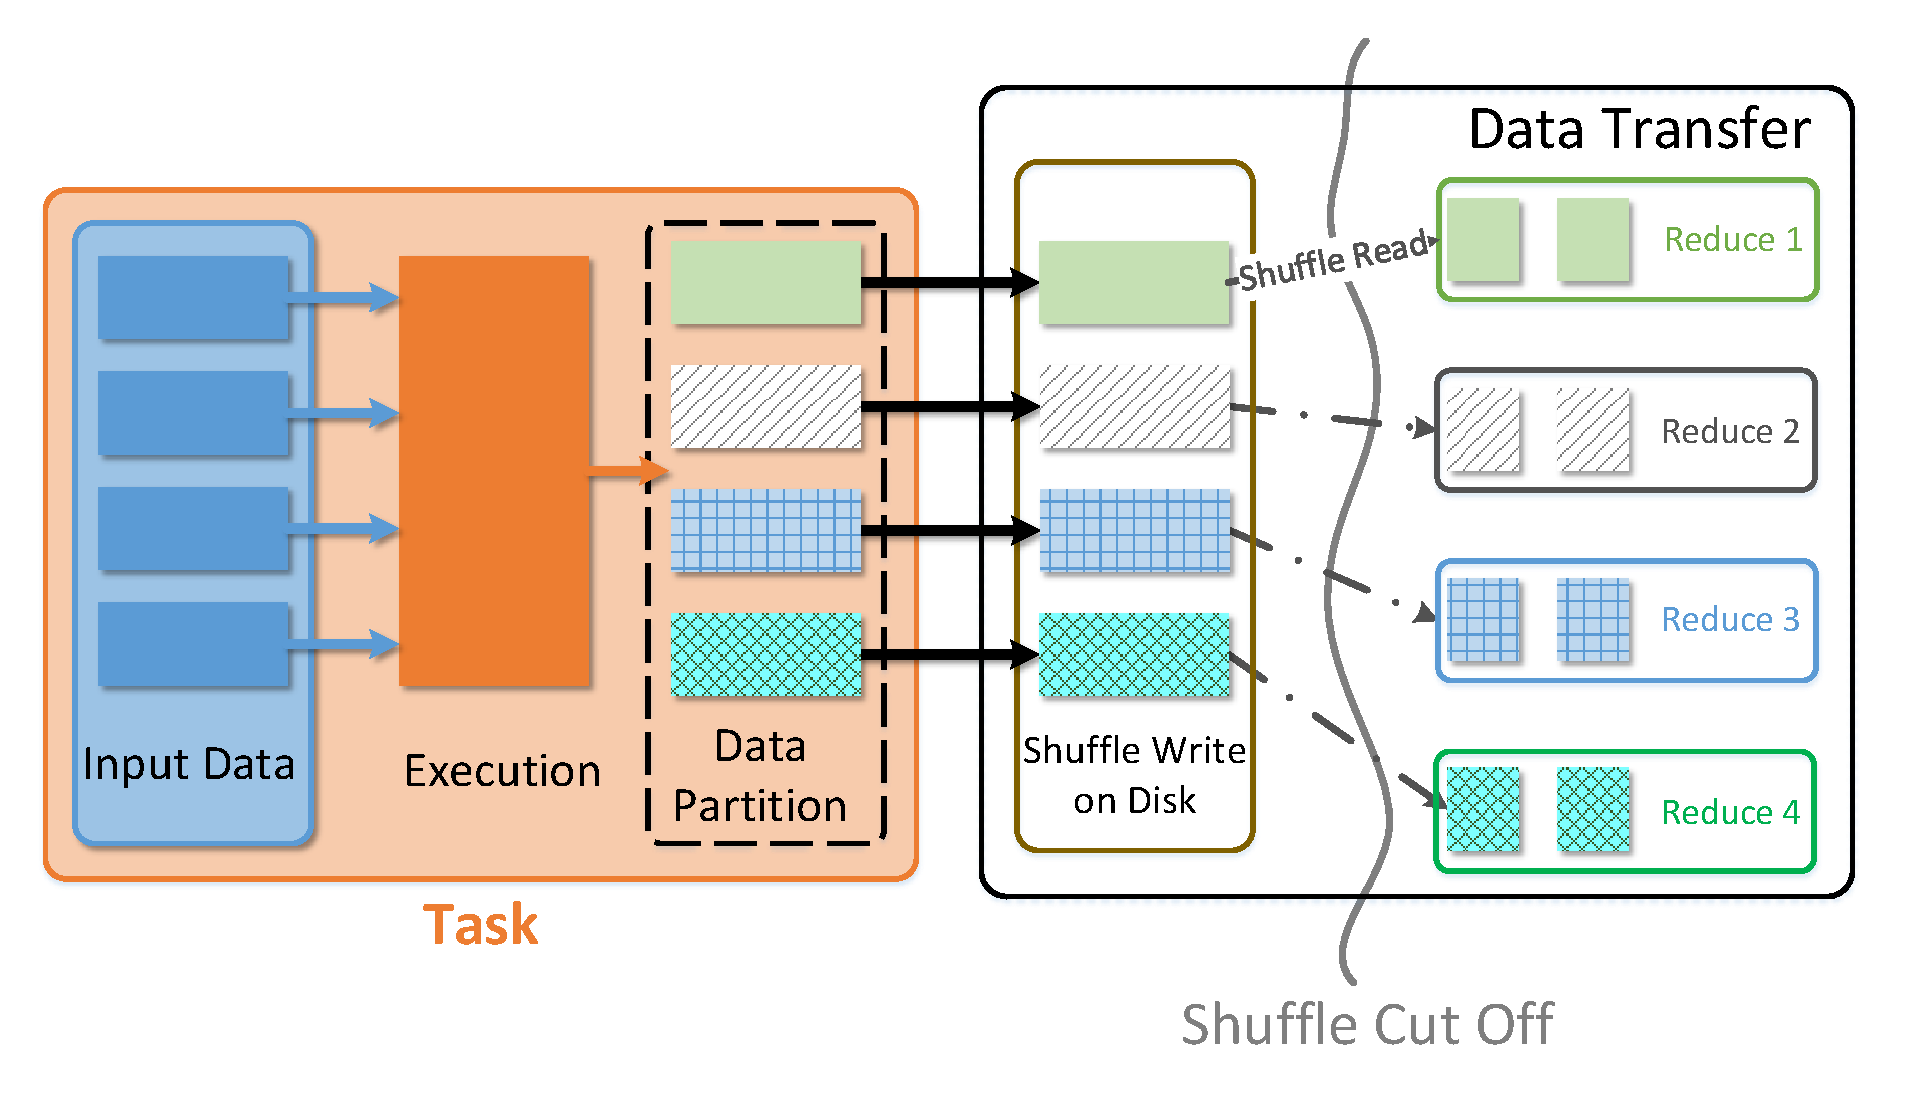
\includegraphics[width=\linewidth]{fig/shuffle_process}
	\caption{Shuffle Overview}
	\label{fig:shuffle_process}
\end{figure}

\begin{figure*}
	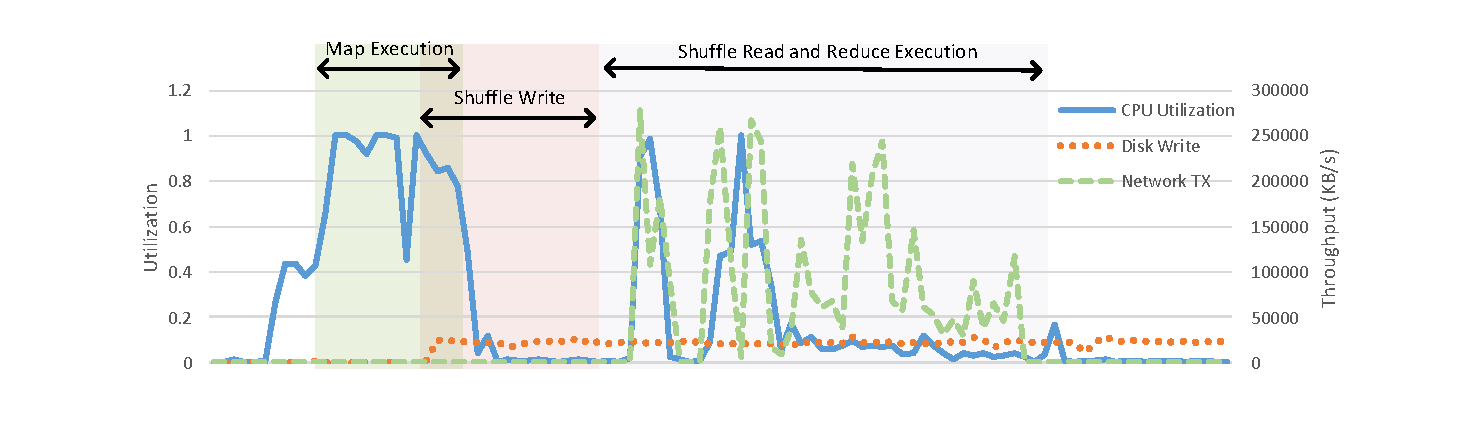
\includegraphics[width=\textwidth]{fig/util}
	\caption{CPU utilization and I/O throughput of a node during a Spark single shuffle application}
	\label{fig:util}
\end{figure*}

\textbf{Impact of shuffle process}. Shuffle process is I/O intensive, which might introduce a significant latency to the application. Reports show that, $60\%$ of MapReduce jobs at Yahoo!
and $20\%$ at Facebook are shuffle intensive \cite{shufflewatcher}. For those shuffle intensive jobs, the shuffle latency may even dominate Job Completion Time (JCT). 
% Is there any definition for "shuffle-intensive"?
For instance, a MapReduce trace analysis from Facebook shows that shuffle accounts for $33\%$ JCT on average, and in shuffle intensive jobs that is up to even $70\%$ \cite{managing}.
Meanwhile, the completion time of shuffle correlates with the performance of storage, network, and even applications. 
This variation may bring a huge challenge for operators to find the correct configuration of the DAG framework.

\subsection{Observations} \label{observation}
Of course, shuffle is unavoidable in a DAG computing process. But \textit{can we mitigate or even remove the overhead of shuffle?} To find the answers, we run some typical Spark applications in a 5-node Amazon EC2 cluster with \texttt{m4.xlarge} instances. We then measure the CPU utilization, I/O throughput and tasks execution information of each node. Take the trace of Spark \textit{GroupByTest} job in Figure \ref{fig:util} as an example. This job has 2 rounds of tasks for each node. We have marked out the execution phase as from the launch time of the first task of this node to the execution finish timestamp of the last one. The \textit{shuffle write} phase is marked from the timestamp of the beginning of the first partitioned data write. The \textit{shuffle read} and \textit{execution} phase is marked from the start of the first reduce launch timestamp.
% Not clear about the marking process.
Figure \ref{fig:util} reveals the performance information of two stages that are connected by shuffle. By analyzing the trace combing with Spark, we propose following observations.


\subsubsection{Multi-rounds tasks in each stages}\label{multi}
Both experience and DAG framework manuals recommend that multi-round execution of each stage will benefit the performance of applications.
For example, Hadoop MapReduce Tutorial \cite{hadooptutorial} suggests that \textit{10-100 maps per-node} and \textit{0.95 or 1.75 $\times$ no. of nodes $\times$ no. of maximum container per node} seem to be the right level of parallelism. Spark Configuration also recommends 2-3 tasks per CPU core in the cluster \cite{sparkconf}.
We have two rounds of tasks in job of Figure \ref{fig:util} to process data of about $70$GB. Figure \ref{fig:util} shows that the second phase of shuffle---\textit{data transfer}---will start until the reduce stage starts.
But the shuffle data will become available as soon as the execution of one task is finished. Though in the context of Spark, the reduce task can do computation while fetching data, the uncontrolled network congestion may still hurt the performance. We have observed that, however, if the destination of the shuffle output of each task can be known in priori, the property of multi-rounds can be leveraged to do \textit{data transfer} ahead of reduce stage.
%This observation is not clearly elaborated. You shall spend more space for it.

\subsubsection{Tight Couple between Shuffle and Computation}
Another information we get from the trace is that, the shuffle process shall be decoupled from task execution. In general, CPU and memory are binded as a computing \textit{slot} by the cluster resource scheduler. When a task is scheduled to a slot, it won't release that slot before completion. In Figure \ref{fig:util}, the resource of Spark executor will be released at the ending of \textit{shuffle write}.
But CPU becomes idle almost as soon as the \textit{execution} is finished. On the other hand, shuffle is I/O intensive. It doesn't involve CPU and application context. If the shuffle can be decoupled from task, the slot can be released after \textit{execution} phase. The early release can benefit other tasks to achieve better overall performance of the DAG framework.

\subsubsection{Variance of I/O Performance}
When we look into the performance of disk and network in our test case, there is huge variance. Since we use the standard EBS as our backend storage for the EC2 instances, the I/O performance of the disk is poor. 
At the same time, the bandwidth of each instance is not specified from Amazon. But the utilization in Figure\ref{fig:util} refers that the bandwidth is about $300$Mbps. In this case, the bottleneck of shuffle is disk, which introduces a significant latency for the application. Vice versa, in some cases, the congestion of network may also become the bottleneck of shuffle \cite{varys}. The uncertainty about the I/O performance causes a huge challenge for optimizing the DAG computing in the cluster. For network latency, the most we can do is to mitigate the transfer delay. As for disk write, we believe it's not necessary for today's cluster. Recall that the persistence of shuffle data is used only for reduce fault tolerance, but the \textit{mean time to failure} (MTTF) for a server is counted in the scale of year \cite{tachyon}. The MTTF is exponential compared with the duration of a shuffle, so we believe the disk write is unnecessary in today's data center. 

\subsubsection{Relatively Small Size of Shuffle Data}\label{shufflesize}
In order to accelerate computation, Spark will put all the input data set for a task into memory. Compared to the input dataset, size of shuffle data is relatively small. We present two typical applications on Spark to compare size of the shuffle data with that of the input data in Figure \ref{fig:shuffle_size}. Although TeraSort \cite{terasort} is known as a shuffle intensive job, in a $10$GB input TeraSort, the shuffle size is less than $3$GB. When it's mapped to a 5-node cluster, it only takes about 500MB memory ($25\%$ of input size for each node) to cache the shuffle data in memory. The data reported in \cite{makingsense} also shows that the amount of data shuffled is less than the input, by as much as a factor of $5-10$. This is another reason that disk should not be involved in the whole shuffle procedure.


Based on these observations, it's straightforward to come up with an optimization that uses memory to store the shuffle data and overlap the I/O operations of shuffle
by leveraging \textit{multi-round} property of DAG computing. In order to achieve this optimization, we have to decouple shuffle from task and 
perform pre-fetch as soon as each output of map task and intermediate task is available. But is this feasible? We try to answer this question
in the following sections.
